% Full-wrap KDP paperback cover (back, spine, front) for a 7 x 10 in trim, black and white interior on white paper.
% Spine = pages x 0.002252 in; full width = 0.125 + 7 + spine + 7 + 0.125 in; height 10.25 in (0.125 in bleed).
% Build it with the page count of the print interior, twice, in this folder:
%   pdflatex "\def\InteriorPages{N}% Full-wrap KDP paperback cover (back, spine, front) for a 7 x 10 in trim, black and white interior on white paper.
% Spine = pages x 0.002252 in; full width = 0.125 + 7 + spine + 7 + 0.125 in; height 10.25 in (0.125 in bleed).
% Build it with the page count of the print interior, twice, in this folder:
%   pdflatex "\def\InteriorPages{N}% Full-wrap KDP paperback cover (back, spine, front) for a 7 x 10 in trim, black and white interior on white paper.
% Spine = pages x 0.002252 in; full width = 0.125 + 7 + spine + 7 + 0.125 in; height 10.25 in (0.125 in bleed).
% Build it with the page count of the print interior, twice, in this folder:
%   pdflatex "\def\InteriorPages{N}% Full-wrap KDP paperback cover (back, spine, front) for a 7 x 10 in trim, black and white interior on white paper.
% Spine = pages x 0.002252 in; full width = 0.125 + 7 + spine + 7 + 0.125 in; height 10.25 in (0.125 in bleed).
% Build it with the page count of the print interior, twice, in this folder:
%   pdflatex "\def\InteriorPages{N}\input{cover}"
% Check it with kdp.py cover <the print interior> --cover cover.pdf (COVER OK), and cut the front cover image for
% the repository and the website with kdp.py front cover.pdf. Without the definition the count below is used.
% KDP prints spine text only on books of more than 79 pages. Keep everything else 0.375 in inside the trim.
% The front is art.png (drawn by art.py, 7.125 x 10.25 in at 400 ppi, no text) with the title, subtitle and authors set over it.
\providecommand\InteriorPages{387}
\documentclass{article}
\usepackage{tikz,graphicx,xcolor}
\pgfmathsetmacro\Spine{\InteriorPages*0.002252}
\pgfmathsetmacro\W{14.25+\Spine}
\pgfmathsetmacro\FrontL{7.125+\Spine}
\pgfmathsetmacro\SpineC{7.125+\Spine/2}
\pgfmathsetmacro\SpineFont{min(14,(\Spine-0.125)*72*0.8)}
\usepackage[paperwidth=\W in,paperheight=10.25in,margin=0in]{geometry}
\usepackage[T1]{fontenc}
\usepackage{tgheros}
\usepackage{microtype}
\renewcommand\familydefault{\sfdefault}
\definecolor{ground}{HTML}{0B1E3A}
\definecolor{paper}{HTML}{E4ECF6}
\definecolor{mist}{HTML}{AEBFD6}
\definecolor{teal}{HTML}{3CC6B5}
\definecolor{amber}{HTML}{F6B26B}
\newcommand\CoverTitle{Clinical Trials in Practice}
\newcommand\SpineAuthors{Sokolova \,\&\, Sokolov}
\pagestyle{empty}
\begin{document}
\noindent\begin{tikzpicture}[x=1in,y=1in,remember picture,overlay,shift={(current page.south west)}]
\fill[ground] (0,0) rectangle (\W,10.25);
% front: the art fills the front panel and its bleed; the text is set over it
\node[anchor=south west,inner sep=0] at (\FrontL,0) {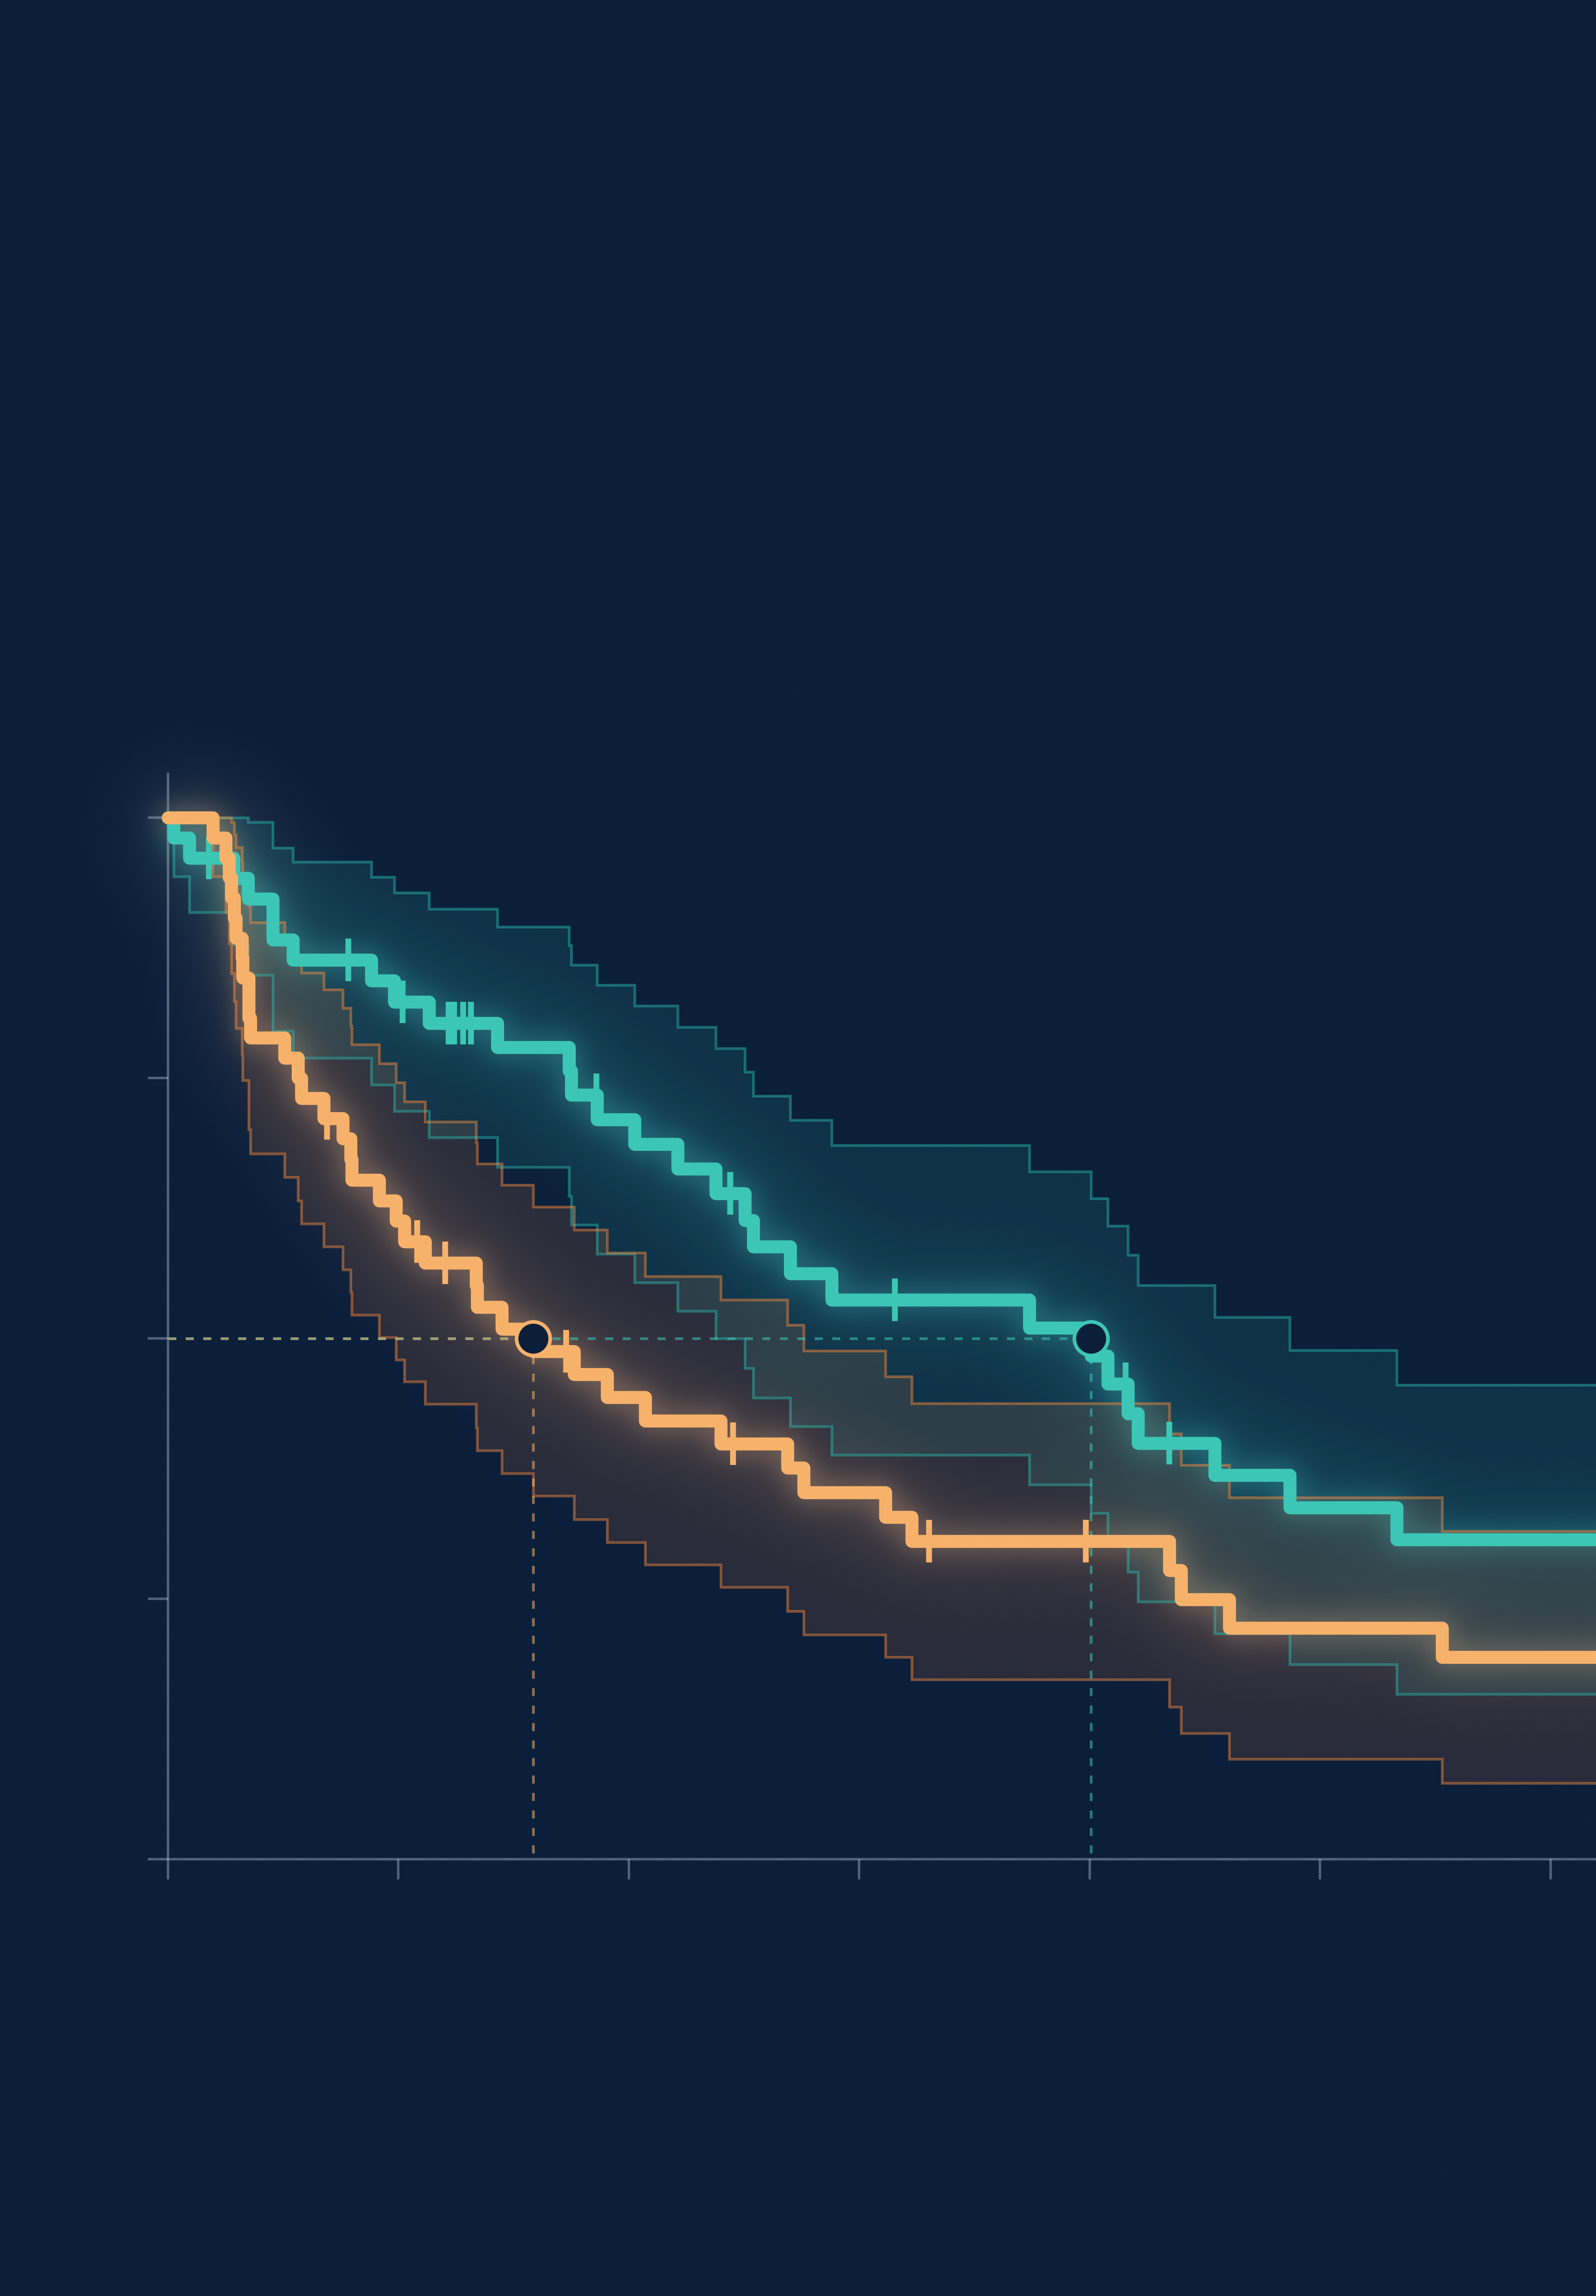
\includegraphics[width=7.125in,height=10.25in]{art.png}};
\begin{scope}[shift={(\FrontL,0)}]
\fill[teal] (0.75,9.66) rectangle (1.25,9.72);
\fill[amber] (1.30,9.66) rectangle (1.80,9.72);
\node[text=white,anchor=base west,inner sep=0] at (0.75,8.78) {\fontsize{62}{66}\selectfont\bfseries Clinical Trials};
\node[text=white,anchor=base west,inner sep=0] at (0.75,7.86) {\fontsize{62}{66}\selectfont\bfseries in Practice};
\node[text=mist,anchor=base west,inner sep=0] at (0.75,7.26) {\fontsize{24}{27}\selectfont From Foundations to AI Agents};
\node[text=white,anchor=base west,inner sep=0] at (0.75,1.38) {\fontsize{22}{25}\selectfont\textls[20]{Alexandra Sokolova}};
\node[text=white,anchor=base west,inner sep=0] at (0.75,0.96) {\fontsize{22}{25}\selectfont\textls[20]{Vadim Sokolov}};
\end{scope}
% spine
\ifnum\InteriorPages>79
\node[text=white,rotate=-90,anchor=center] at (\SpineC,6.3) {\fontsize{\SpineFont}{\SpineFont}\selectfont\bfseries\CoverTitle};
\node[text=teal,rotate=-90,anchor=center] at (\SpineC,1.9) {\fontsize{\SpineFont}{\SpineFont}\selectfont\bfseries\SpineAuthors};
\fi
% back
\fill[teal] (0.75,9.66) rectangle (1.25,9.72);
\fill[amber] (1.30,9.66) rectangle (1.80,9.72);
\node[text=paper,anchor=north west,inner sep=0,text width=5.6in,align=justify] at (0.75,9.36) {%
\fontsize{11.25}{15.2}\selectfont\frenchspacing
{\fontsize{19}{23}\selectfont\bfseries\color{teal}\raggedright From the first protocol draft\\to regulatory submission\par}
\vspace{0.9em}
\looseness=-1 Clinical trials are how medicine finds out what works. They are slow, expensive, and tightly regulated, and a poorly run trial can hide a real benefit or miss a serious harm.\par
\vspace{0.7em}
This book treats clinical trials as science and as regulated operations, and gives Phase III the most room, because that is where approval is won or lost. It covers the phases, statistical foundations, adaptive and Bayesian design, the daily work of a study from sites and recruitment to data management, monitoring, and safety, and the path from closeout through the clinical study report to submission.\par
\vspace{0.7em}
Where it turns to automation and AI agents, one test applies: the tool must stand up in an inspection, with validation, governance, and a named person accountable for each decision.\par
\vspace{0.7em}
Alexandra Sokolova is at Oregon Health and Science University. Vadim Sokolov is at George Mason University.\par
};
% barcode area, kept clear: KDP prints the barcode here
\fill[white] (4.875,0.375) rectangle (6.875,1.575);
\end{tikzpicture}
\end{document}
"
% Check it with kdp.py cover <the print interior> --cover cover.pdf (COVER OK), and cut the front cover image for
% the repository and the website with kdp.py front cover.pdf. Without the definition the count below is used.
% KDP prints spine text only on books of more than 79 pages. Keep everything else 0.375 in inside the trim.
% The front is art.png (drawn by art.py, 7.125 x 10.25 in at 400 ppi, no text) with the title, subtitle and authors set over it.
\providecommand\InteriorPages{387}
\documentclass{article}
\usepackage{tikz,graphicx,xcolor}
\pgfmathsetmacro\Spine{\InteriorPages*0.002252}
\pgfmathsetmacro\W{14.25+\Spine}
\pgfmathsetmacro\FrontL{7.125+\Spine}
\pgfmathsetmacro\SpineC{7.125+\Spine/2}
\pgfmathsetmacro\SpineFont{min(14,(\Spine-0.125)*72*0.8)}
\usepackage[paperwidth=\W in,paperheight=10.25in,margin=0in]{geometry}
\usepackage[T1]{fontenc}
\usepackage{tgheros}
\usepackage{microtype}
\renewcommand\familydefault{\sfdefault}
\definecolor{ground}{HTML}{0B1E3A}
\definecolor{paper}{HTML}{E4ECF6}
\definecolor{mist}{HTML}{AEBFD6}
\definecolor{teal}{HTML}{3CC6B5}
\definecolor{amber}{HTML}{F6B26B}
\newcommand\CoverTitle{Clinical Trials in Practice}
\newcommand\SpineAuthors{Sokolova \,\&\, Sokolov}
\pagestyle{empty}
\begin{document}
\noindent\begin{tikzpicture}[x=1in,y=1in,remember picture,overlay,shift={(current page.south west)}]
\fill[ground] (0,0) rectangle (\W,10.25);
% front: the art fills the front panel and its bleed; the text is set over it
\node[anchor=south west,inner sep=0] at (\FrontL,0) {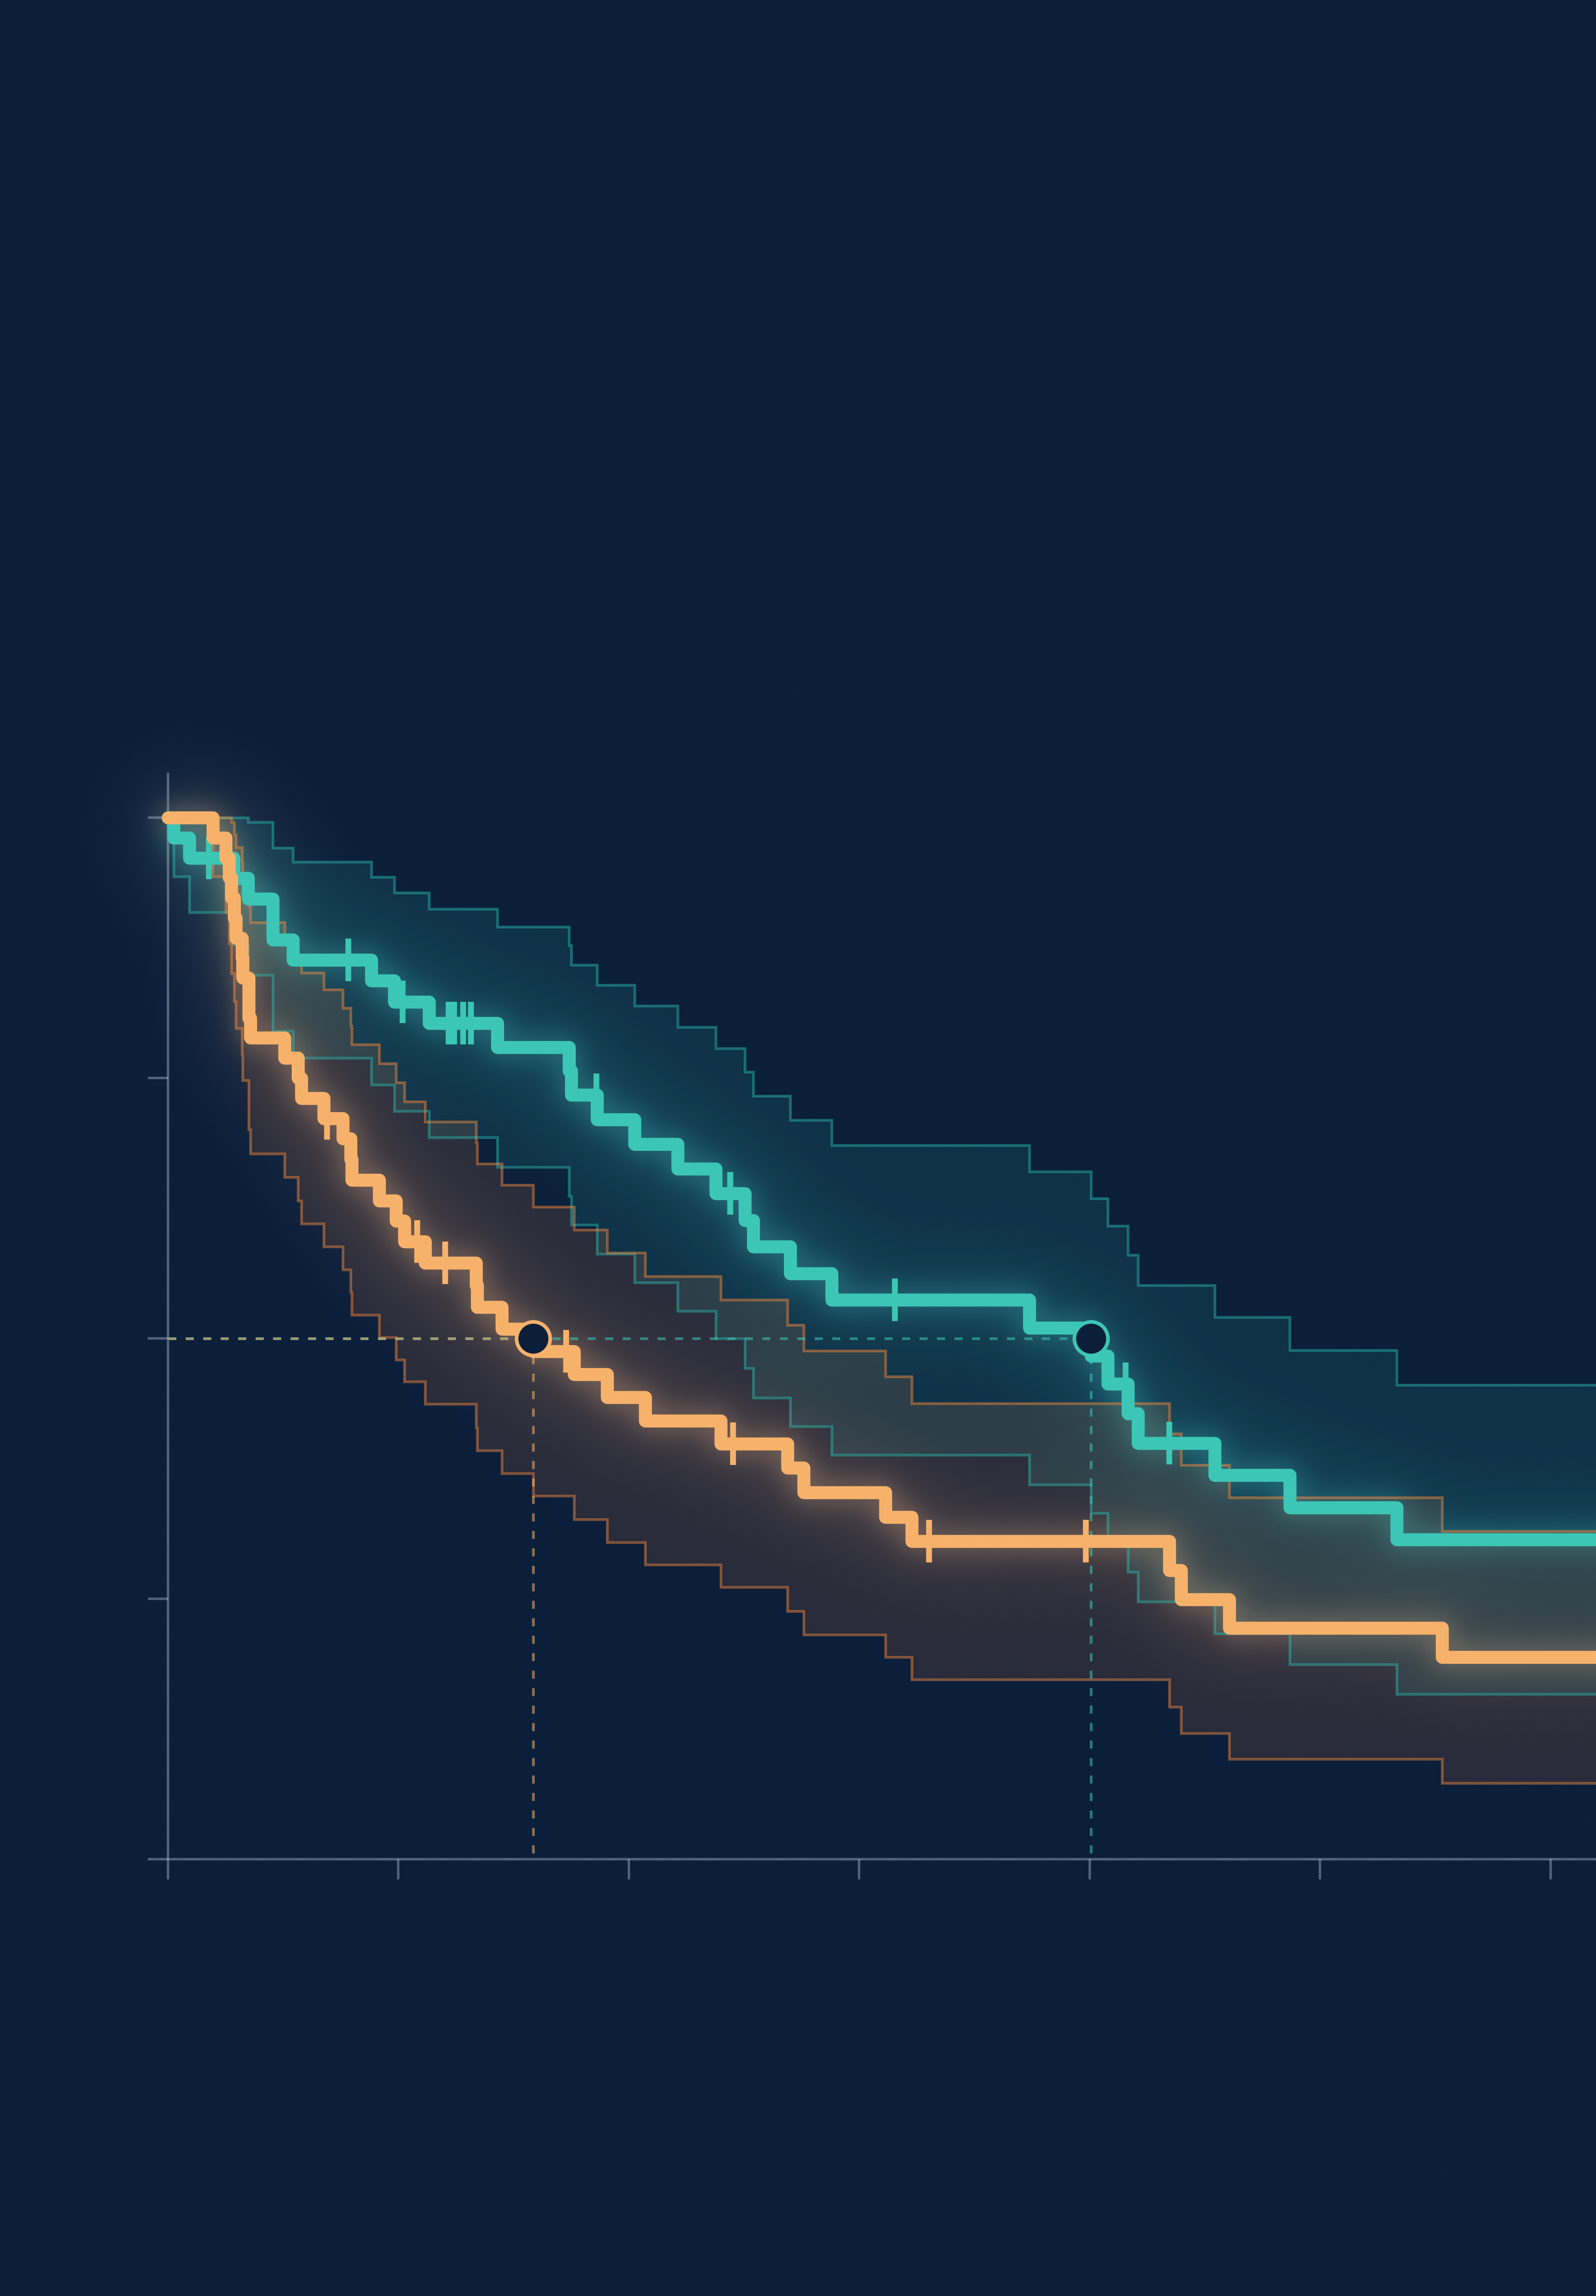
\includegraphics[width=7.125in,height=10.25in]{art.png}};
\begin{scope}[shift={(\FrontL,0)}]
\fill[teal] (0.75,9.66) rectangle (1.25,9.72);
\fill[amber] (1.30,9.66) rectangle (1.80,9.72);
\node[text=white,anchor=base west,inner sep=0] at (0.75,8.78) {\fontsize{62}{66}\selectfont\bfseries Clinical Trials};
\node[text=white,anchor=base west,inner sep=0] at (0.75,7.86) {\fontsize{62}{66}\selectfont\bfseries in Practice};
\node[text=mist,anchor=base west,inner sep=0] at (0.75,7.26) {\fontsize{24}{27}\selectfont From Foundations to AI Agents};
\node[text=white,anchor=base west,inner sep=0] at (0.75,1.38) {\fontsize{22}{25}\selectfont\textls[20]{Alexandra Sokolova}};
\node[text=white,anchor=base west,inner sep=0] at (0.75,0.96) {\fontsize{22}{25}\selectfont\textls[20]{Vadim Sokolov}};
\end{scope}
% spine
\ifnum\InteriorPages>79
\node[text=white,rotate=-90,anchor=center] at (\SpineC,6.3) {\fontsize{\SpineFont}{\SpineFont}\selectfont\bfseries\CoverTitle};
\node[text=teal,rotate=-90,anchor=center] at (\SpineC,1.9) {\fontsize{\SpineFont}{\SpineFont}\selectfont\bfseries\SpineAuthors};
\fi
% back
\fill[teal] (0.75,9.66) rectangle (1.25,9.72);
\fill[amber] (1.30,9.66) rectangle (1.80,9.72);
\node[text=paper,anchor=north west,inner sep=0,text width=5.6in,align=justify] at (0.75,9.36) {%
\fontsize{11.25}{15.2}\selectfont\frenchspacing
{\fontsize{19}{23}\selectfont\bfseries\color{teal}\raggedright From the first protocol draft\\to regulatory submission\par}
\vspace{0.9em}
\looseness=-1 Clinical trials are how medicine finds out what works. They are slow, expensive, and tightly regulated, and a poorly run trial can hide a real benefit or miss a serious harm.\par
\vspace{0.7em}
This book treats clinical trials as science and as regulated operations, and gives Phase III the most room, because that is where approval is won or lost. It covers the phases, statistical foundations, adaptive and Bayesian design, the daily work of a study from sites and recruitment to data management, monitoring, and safety, and the path from closeout through the clinical study report to submission.\par
\vspace{0.7em}
Where it turns to automation and AI agents, one test applies: the tool must stand up in an inspection, with validation, governance, and a named person accountable for each decision.\par
\vspace{0.7em}
Alexandra Sokolova is at Oregon Health and Science University. Vadim Sokolov is at George Mason University.\par
};
% barcode area, kept clear: KDP prints the barcode here
\fill[white] (4.875,0.375) rectangle (6.875,1.575);
\end{tikzpicture}
\end{document}
"
% Check it with kdp.py cover <the print interior> --cover cover.pdf (COVER OK), and cut the front cover image for
% the repository and the website with kdp.py front cover.pdf. Without the definition the count below is used.
% KDP prints spine text only on books of more than 79 pages. Keep everything else 0.375 in inside the trim.
% The front is art.png (drawn by art.py, 7.125 x 10.25 in at 400 ppi, no text) with the title, subtitle and authors set over it.
\providecommand\InteriorPages{387}
\documentclass{article}
\usepackage{tikz,graphicx,xcolor}
\pgfmathsetmacro\Spine{\InteriorPages*0.002252}
\pgfmathsetmacro\W{14.25+\Spine}
\pgfmathsetmacro\FrontL{7.125+\Spine}
\pgfmathsetmacro\SpineC{7.125+\Spine/2}
\pgfmathsetmacro\SpineFont{min(14,(\Spine-0.125)*72*0.8)}
\usepackage[paperwidth=\W in,paperheight=10.25in,margin=0in]{geometry}
\usepackage[T1]{fontenc}
\usepackage{tgheros}
\usepackage{microtype}
\renewcommand\familydefault{\sfdefault}
\definecolor{ground}{HTML}{0B1E3A}
\definecolor{paper}{HTML}{E4ECF6}
\definecolor{mist}{HTML}{AEBFD6}
\definecolor{teal}{HTML}{3CC6B5}
\definecolor{amber}{HTML}{F6B26B}
\newcommand\CoverTitle{Clinical Trials in Practice}
\newcommand\SpineAuthors{Sokolova \,\&\, Sokolov}
\pagestyle{empty}
\begin{document}
\noindent\begin{tikzpicture}[x=1in,y=1in,remember picture,overlay,shift={(current page.south west)}]
\fill[ground] (0,0) rectangle (\W,10.25);
% front: the art fills the front panel and its bleed; the text is set over it
\node[anchor=south west,inner sep=0] at (\FrontL,0) {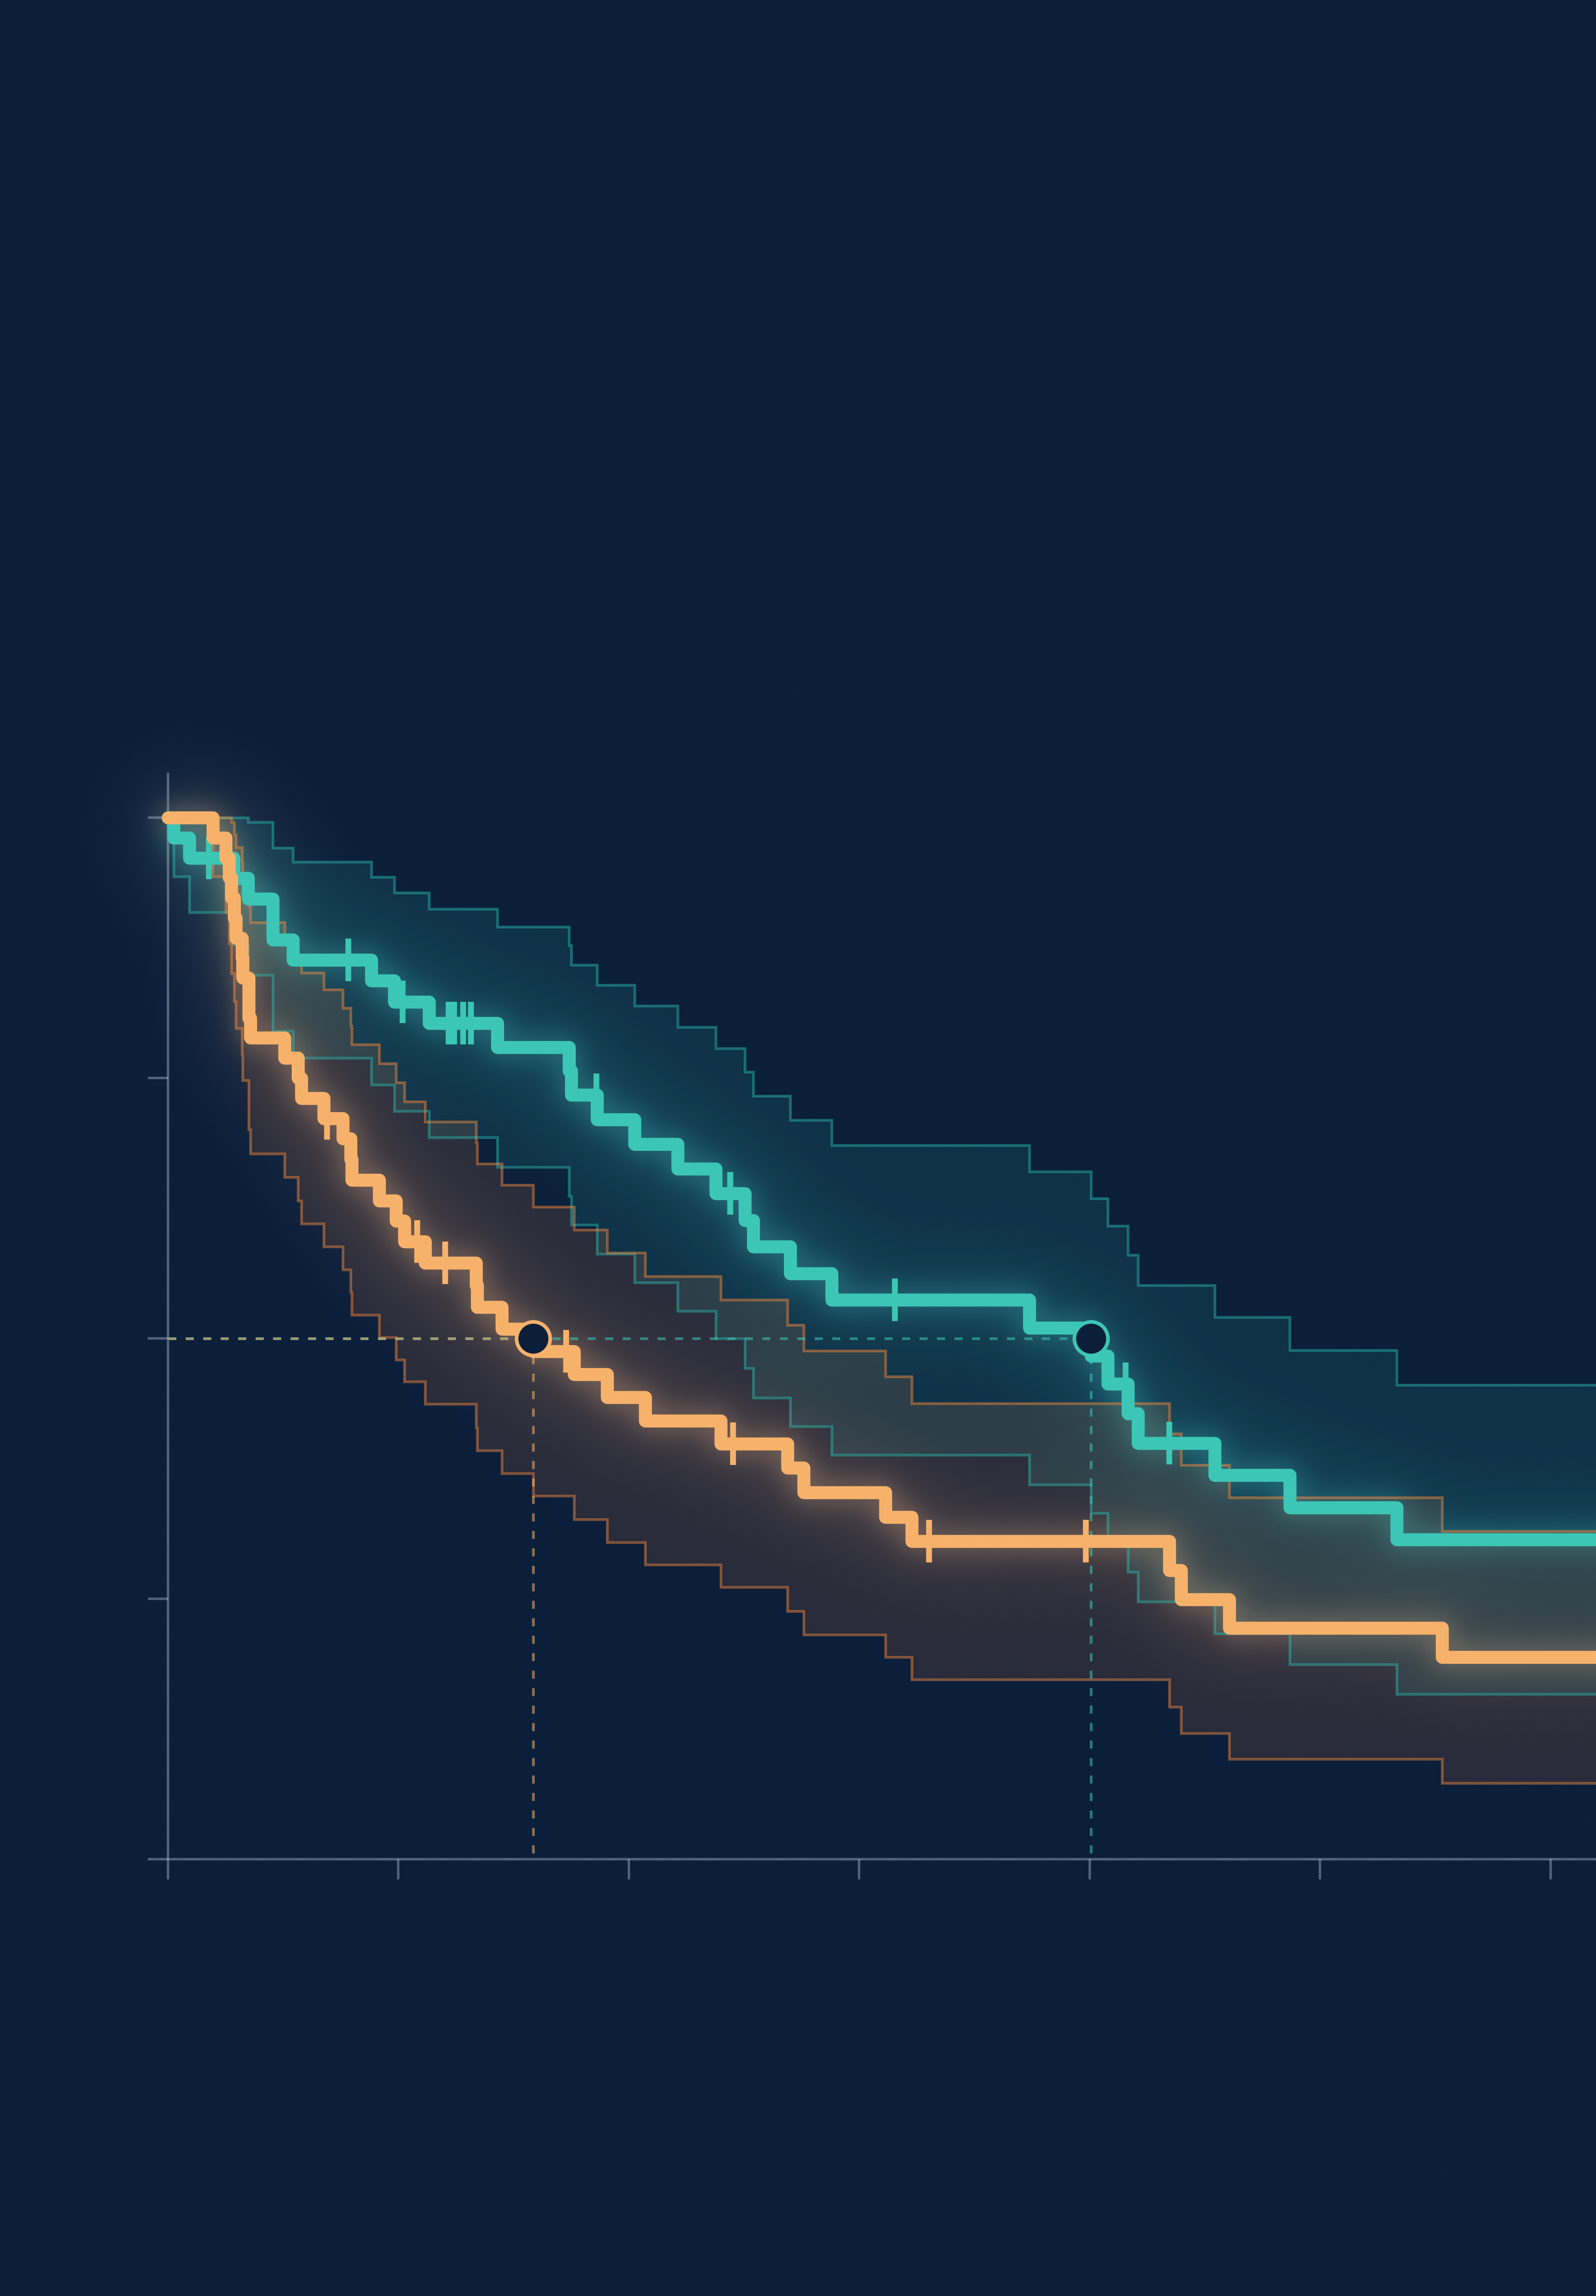
\includegraphics[width=7.125in,height=10.25in]{art.png}};
\begin{scope}[shift={(\FrontL,0)}]
\fill[teal] (0.75,9.66) rectangle (1.25,9.72);
\fill[amber] (1.30,9.66) rectangle (1.80,9.72);
\node[text=white,anchor=base west,inner sep=0] at (0.75,8.78) {\fontsize{62}{66}\selectfont\bfseries Clinical Trials};
\node[text=white,anchor=base west,inner sep=0] at (0.75,7.86) {\fontsize{62}{66}\selectfont\bfseries in Practice};
\node[text=mist,anchor=base west,inner sep=0] at (0.75,7.26) {\fontsize{24}{27}\selectfont From Foundations to AI Agents};
\node[text=white,anchor=base west,inner sep=0] at (0.75,1.38) {\fontsize{22}{25}\selectfont\textls[20]{Alexandra Sokolova}};
\node[text=white,anchor=base west,inner sep=0] at (0.75,0.96) {\fontsize{22}{25}\selectfont\textls[20]{Vadim Sokolov}};
\end{scope}
% spine
\ifnum\InteriorPages>79
\node[text=white,rotate=-90,anchor=center] at (\SpineC,6.3) {\fontsize{\SpineFont}{\SpineFont}\selectfont\bfseries\CoverTitle};
\node[text=teal,rotate=-90,anchor=center] at (\SpineC,1.9) {\fontsize{\SpineFont}{\SpineFont}\selectfont\bfseries\SpineAuthors};
\fi
% back
\fill[teal] (0.75,9.66) rectangle (1.25,9.72);
\fill[amber] (1.30,9.66) rectangle (1.80,9.72);
\node[text=paper,anchor=north west,inner sep=0,text width=5.6in,align=justify] at (0.75,9.36) {%
\fontsize{11.25}{15.2}\selectfont\frenchspacing
{\fontsize{19}{23}\selectfont\bfseries\color{teal}\raggedright From the first protocol draft\\to regulatory submission\par}
\vspace{0.9em}
\looseness=-1 Clinical trials are how medicine finds out what works. They are slow, expensive, and tightly regulated, and a poorly run trial can hide a real benefit or miss a serious harm.\par
\vspace{0.7em}
This book treats clinical trials as science and as regulated operations, and gives Phase III the most room, because that is where approval is won or lost. It covers the phases, statistical foundations, adaptive and Bayesian design, the daily work of a study from sites and recruitment to data management, monitoring, and safety, and the path from closeout through the clinical study report to submission.\par
\vspace{0.7em}
Where it turns to automation and AI agents, one test applies: the tool must stand up in an inspection, with validation, governance, and a named person accountable for each decision.\par
\vspace{0.7em}
Alexandra Sokolova is at Oregon Health and Science University. Vadim Sokolov is at George Mason University.\par
};
% barcode area, kept clear: KDP prints the barcode here
\fill[white] (4.875,0.375) rectangle (6.875,1.575);
\end{tikzpicture}
\end{document}
"
% Check it with kdp.py cover <the print interior> --cover cover.pdf (COVER OK), and cut the front cover image for
% the repository and the website with kdp.py front cover.pdf. Without the definition the count below is used.
% KDP prints spine text only on books of more than 79 pages. Keep everything else 0.375 in inside the trim.
% The front is art.png (drawn by art.py, 7.125 x 10.25 in at 400 ppi, no text) with the title, subtitle and authors set over it.
\providecommand\InteriorPages{387}
\documentclass{article}
\usepackage{tikz,graphicx,xcolor}
\pgfmathsetmacro\Spine{\InteriorPages*0.002252}
\pgfmathsetmacro\W{14.25+\Spine}
\pgfmathsetmacro\FrontL{7.125+\Spine}
\pgfmathsetmacro\SpineC{7.125+\Spine/2}
\pgfmathsetmacro\SpineFont{min(14,(\Spine-0.125)*72*0.8)}
\usepackage[paperwidth=\W in,paperheight=10.25in,margin=0in]{geometry}
\usepackage[T1]{fontenc}
\usepackage{tgheros}
\usepackage{microtype}
\renewcommand\familydefault{\sfdefault}
\definecolor{ground}{HTML}{0B1E3A}
\definecolor{paper}{HTML}{E4ECF6}
\definecolor{mist}{HTML}{AEBFD6}
\definecolor{teal}{HTML}{3CC6B5}
\definecolor{amber}{HTML}{F6B26B}
\newcommand\CoverTitle{Clinical Trials in Practice}
\newcommand\SpineAuthors{Sokolova \,\&\, Sokolov}
\pagestyle{empty}
\begin{document}
\noindent\begin{tikzpicture}[x=1in,y=1in,remember picture,overlay,shift={(current page.south west)}]
\fill[ground] (0,0) rectangle (\W,10.25);
% front: the art fills the front panel and its bleed; the text is set over it
\node[anchor=south west,inner sep=0] at (\FrontL,0) {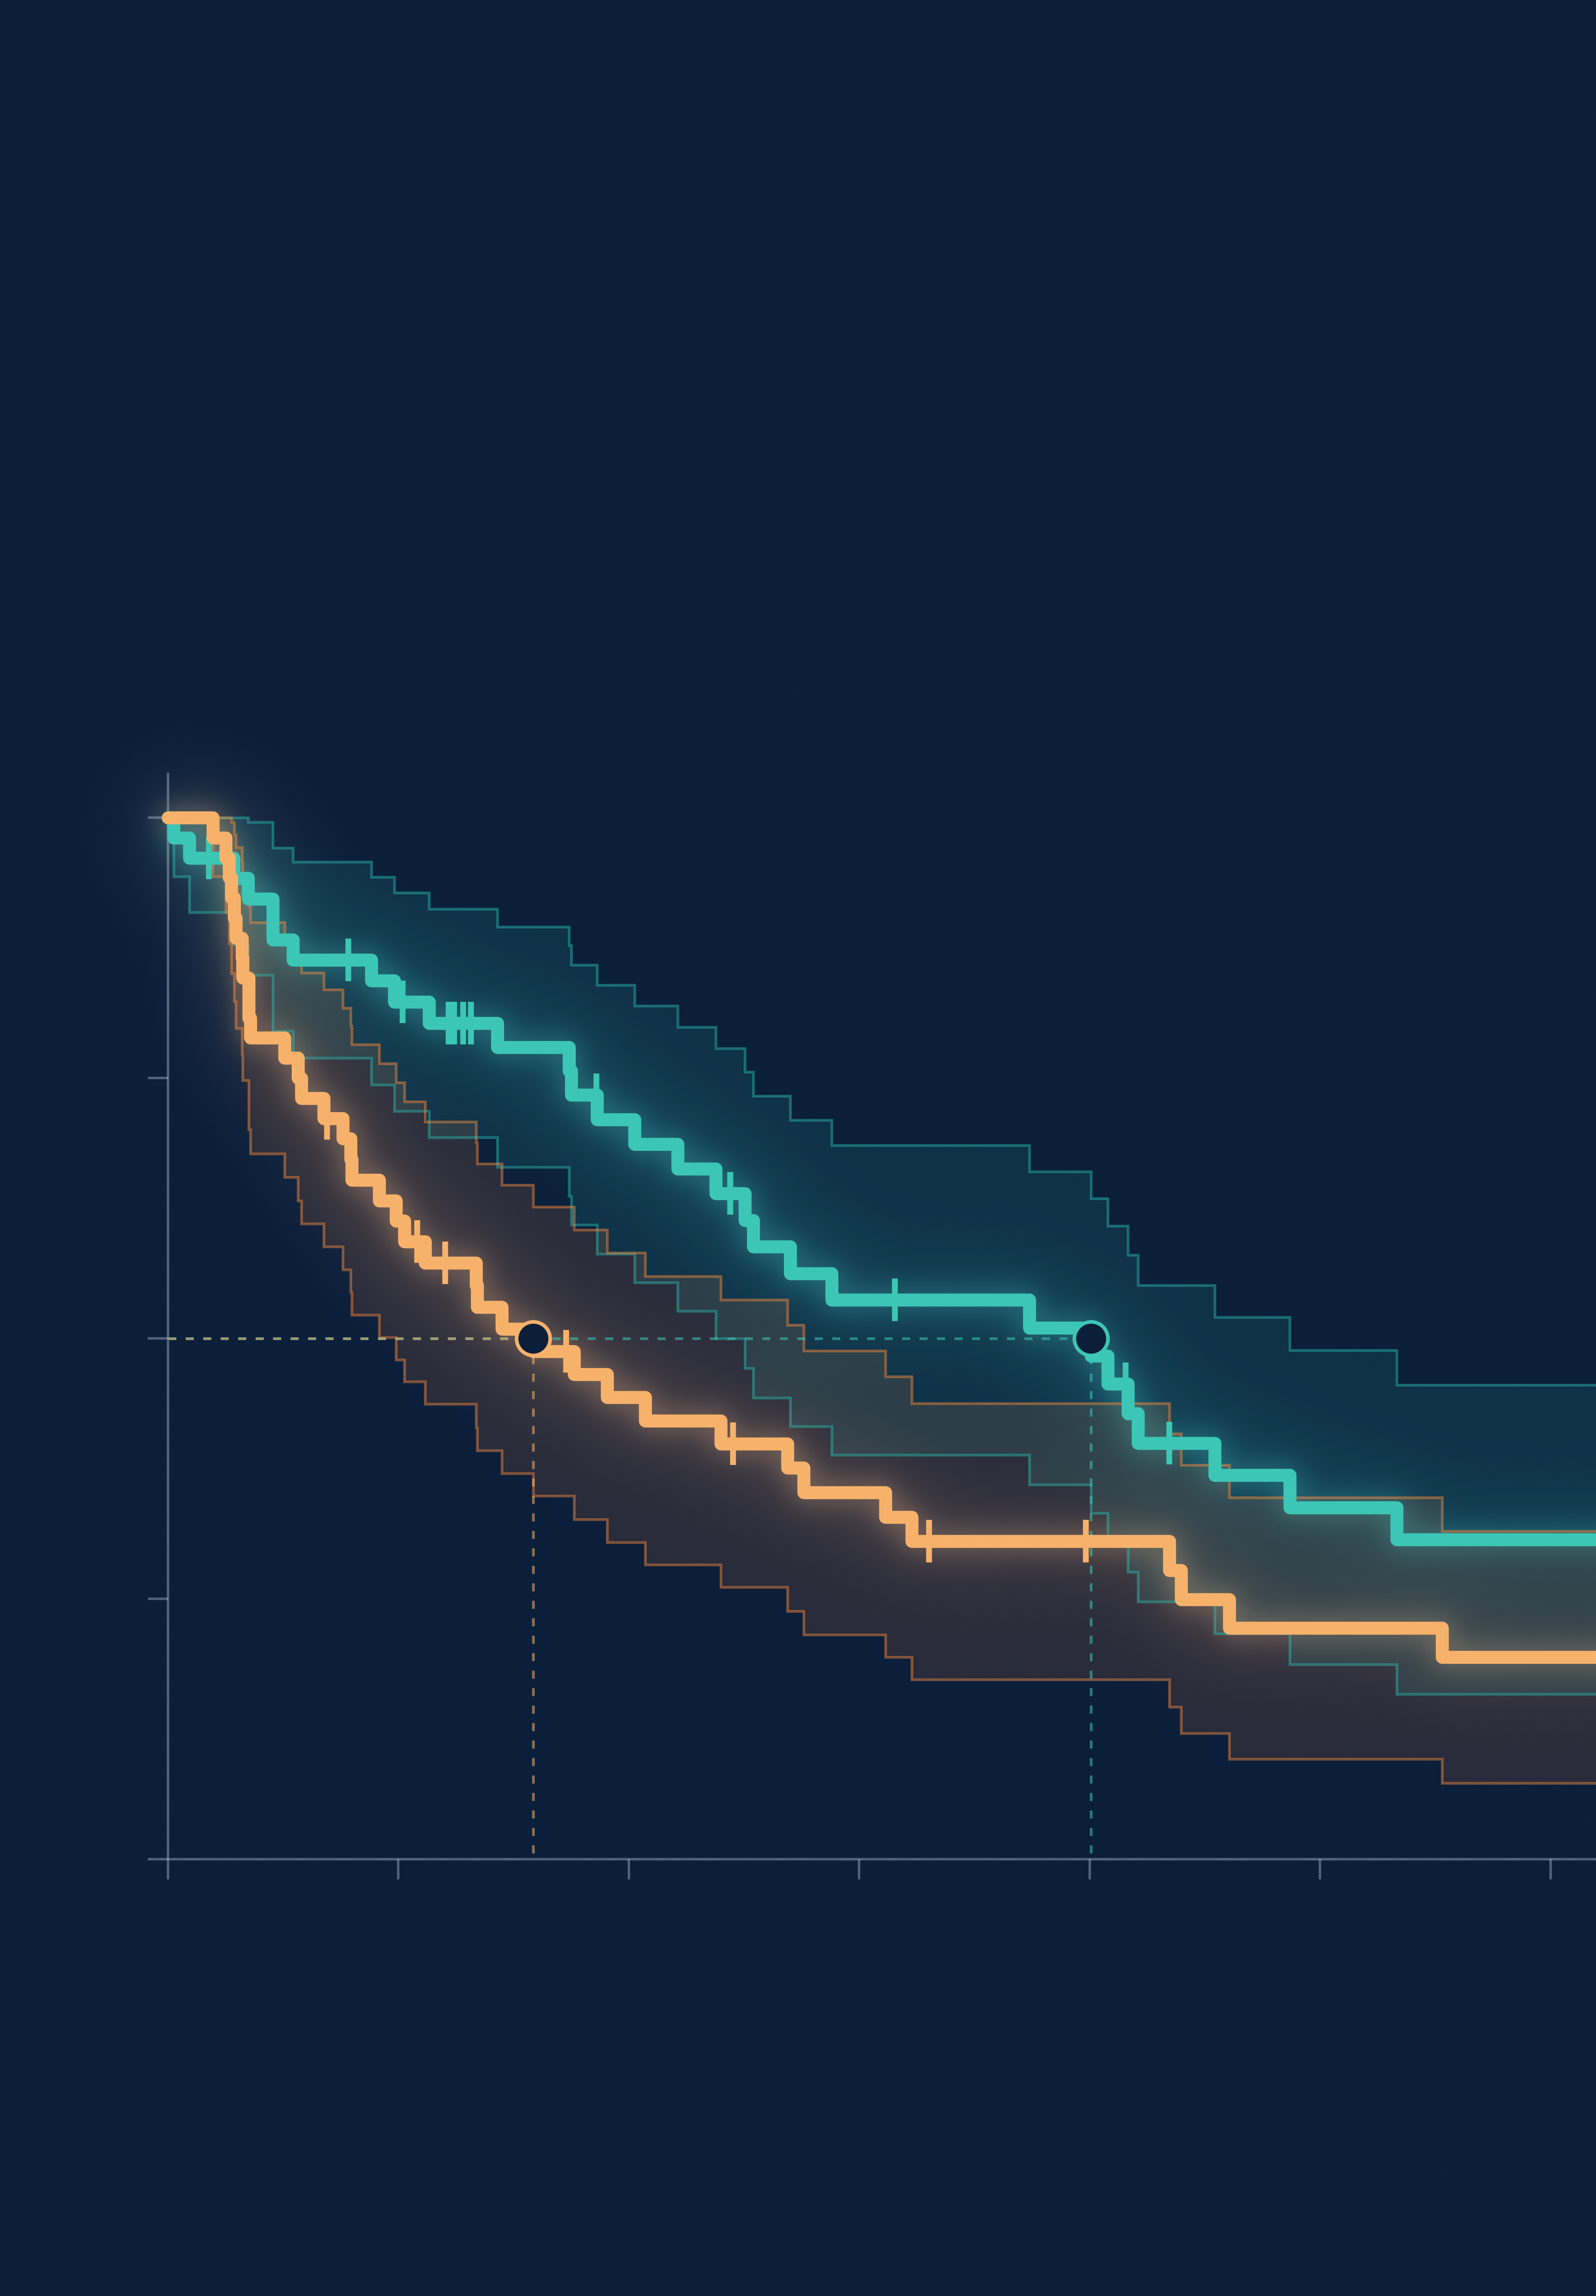
\includegraphics[width=7.125in,height=10.25in]{art.png}};
\begin{scope}[shift={(\FrontL,0)}]
\fill[teal] (0.75,9.66) rectangle (1.25,9.72);
\fill[amber] (1.30,9.66) rectangle (1.80,9.72);
\node[text=white,anchor=base west,inner sep=0] at (0.75,8.78) {\fontsize{62}{66}\selectfont\bfseries Clinical Trials};
\node[text=white,anchor=base west,inner sep=0] at (0.75,7.86) {\fontsize{62}{66}\selectfont\bfseries in Practice};
\node[text=mist,anchor=base west,inner sep=0] at (0.75,7.26) {\fontsize{24}{27}\selectfont From Foundations to AI Agents};
\node[text=white,anchor=base west,inner sep=0] at (0.75,1.38) {\fontsize{22}{25}\selectfont\textls[20]{Alexandra Sokolova}};
\node[text=white,anchor=base west,inner sep=0] at (0.75,0.96) {\fontsize{22}{25}\selectfont\textls[20]{Vadim Sokolov}};
\end{scope}
% spine
\ifnum\InteriorPages>79
\node[text=white,rotate=-90,anchor=center] at (\SpineC,6.3) {\fontsize{\SpineFont}{\SpineFont}\selectfont\bfseries\CoverTitle};
\node[text=teal,rotate=-90,anchor=center] at (\SpineC,1.9) {\fontsize{\SpineFont}{\SpineFont}\selectfont\bfseries\SpineAuthors};
\fi
% back
\fill[teal] (0.75,9.66) rectangle (1.25,9.72);
\fill[amber] (1.30,9.66) rectangle (1.80,9.72);
\node[text=paper,anchor=north west,inner sep=0,text width=5.6in,align=justify] at (0.75,9.36) {%
\fontsize{11.25}{15.2}\selectfont\frenchspacing
{\fontsize{19}{23}\selectfont\bfseries\color{teal}\raggedright From the first protocol draft\\to regulatory submission\par}
\vspace{0.9em}
\looseness=-1 Clinical trials are how medicine finds out what works. They are slow, expensive, and tightly regulated, and a poorly run trial can hide a real benefit or miss a serious harm.\par
\vspace{0.7em}
This book treats clinical trials as science and as regulated operations, and gives Phase III the most room, because that is where approval is won or lost. It covers the phases, statistical foundations, adaptive and Bayesian design, the daily work of a study from sites and recruitment to data management, monitoring, and safety, and the path from closeout through the clinical study report to submission.\par
\vspace{0.7em}
Where it turns to automation and AI agents, one test applies: the tool must stand up in an inspection, with validation, governance, and a named person accountable for each decision.\par
\vspace{0.7em}
Alexandra Sokolova is at Oregon Health and Science University. Vadim Sokolov is at George Mason University.\par
};
% barcode area, kept clear: KDP prints the barcode here
\fill[white] (4.875,0.375) rectangle (6.875,1.575);
\end{tikzpicture}
\end{document}
